\section{The complete positive source and its exact
quotient}\label{the-complete-positive-source-and-its-exact-quotient}

The following complete proofs calculate positivity before quotienting
the original arithmetic source. SPF proves that every continuous
positive transfer-adjoint form on that source is represented by a unique
positive measure of polynomial growth. Its Gaussian cyclicity argument
derives the scalar measure representation rather than assuming it.
Direct descent through the full original ideal is exactly support on the
actual critical-line zero set.

SMC then proves the exact closure of the original summation image for
every such measure. It constructs the completed quotient, its
original-source kernel, full involution, original degree action and all
bounded changes of measure. The ordinary Mellin density is the earlier
M9 result; its complete constants are retained in the comparison. The
new simultaneous continuous and atomic receiver gives the exact effect
on AST's actual specialization row, with the full original Weil
complement still present.

\begin{figure}
\centering
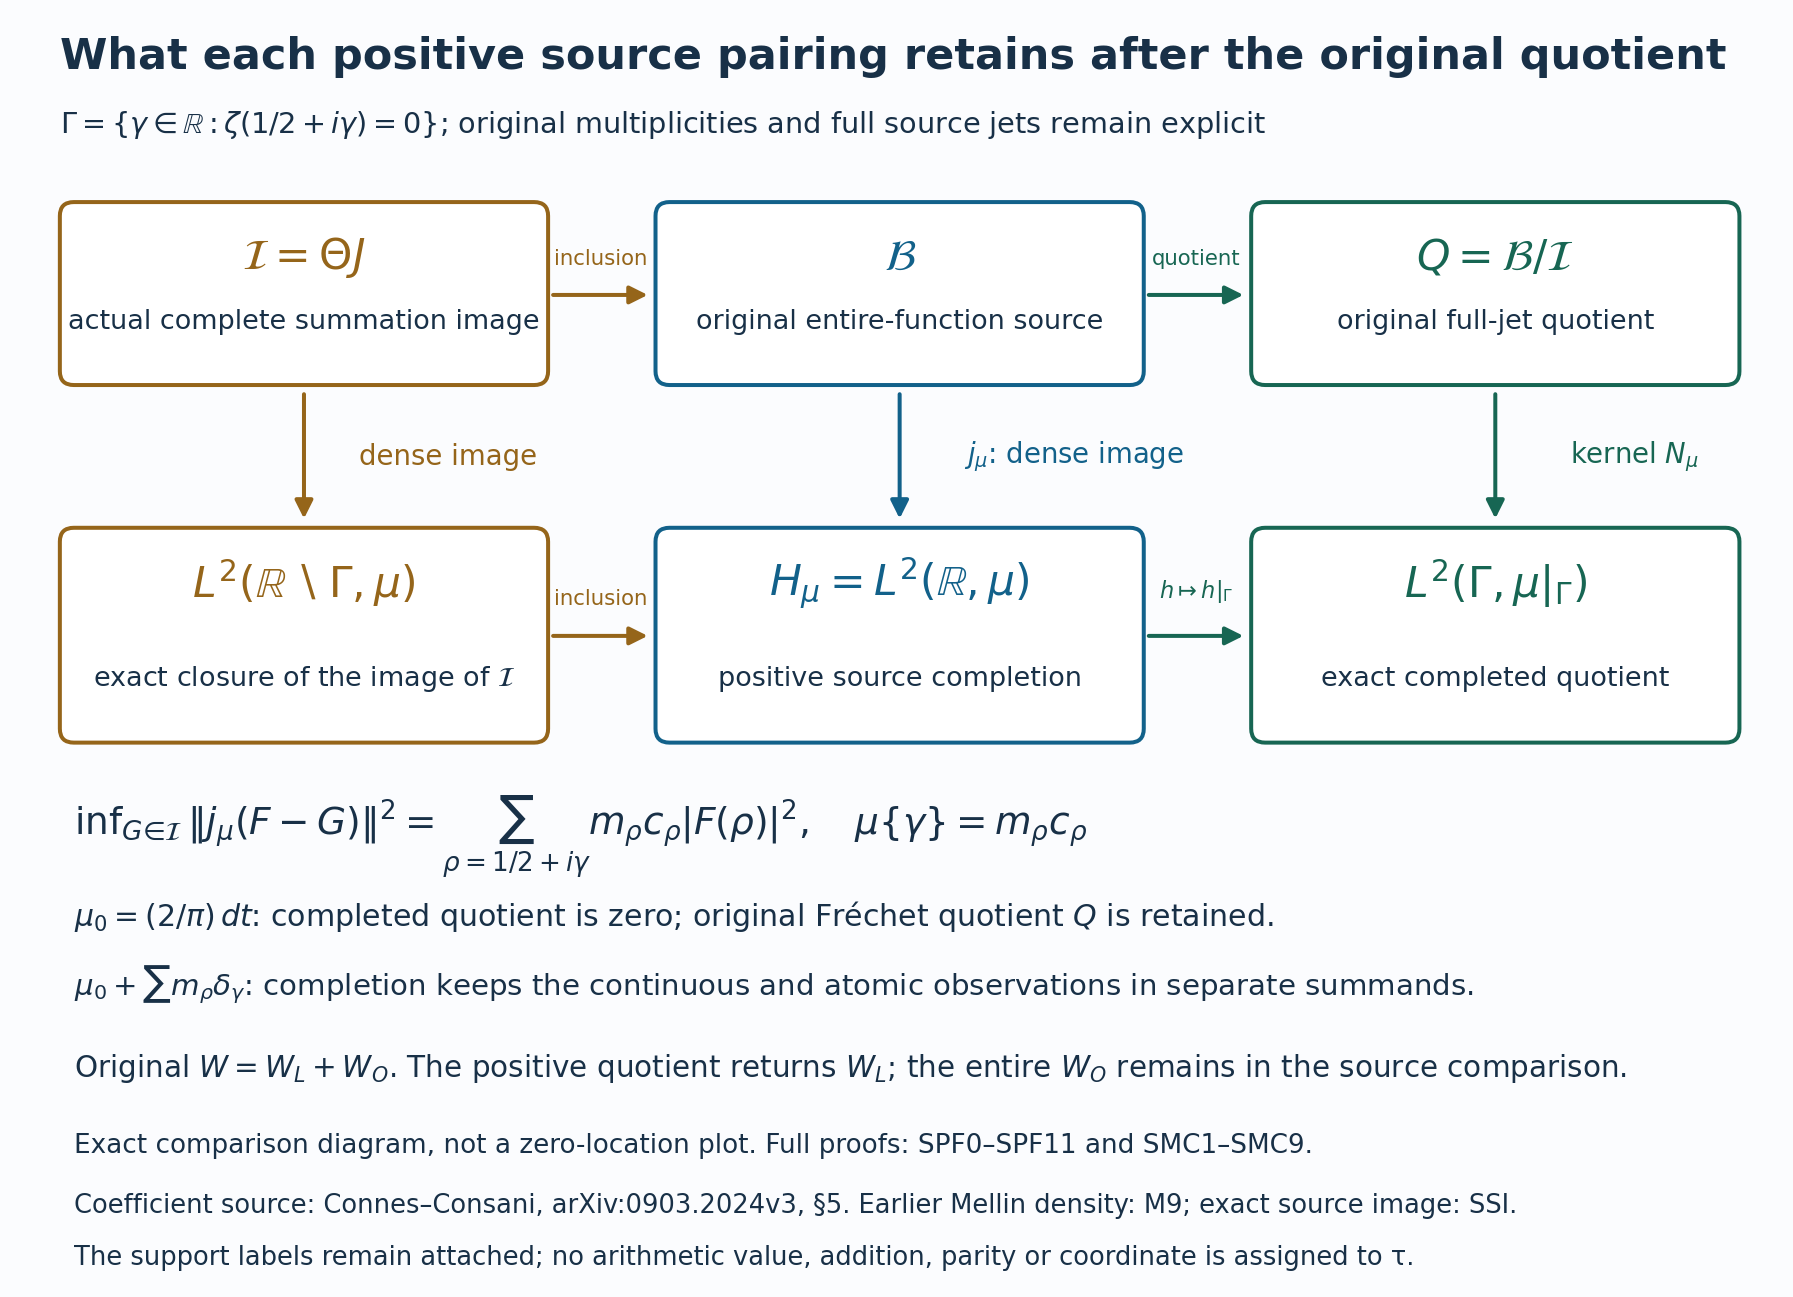
\includegraphics[width=1\linewidth,height=\textheight,keepaspectratio,alt={The two exact rows compare the original full-jet source and its measure completion. SMC1 proves both dense source images; SMC3 proves the lower closed image and orthogonal quotient; SMC4 gives the full kernel and quotient norm. SMC5 retains the actual involution and cover degrees. The lower quotient records only atoms at original line zeros, with every multiplicity displayed. The original source still retains all higher jets and possible off-line blocks. This is a comparison of exact maps, not a numerical zero-location plot.}]{source_measure_quotient.png}
\caption{The two exact rows compare the original full-jet source and its
measure completion. SMC1 proves both dense source images; SMC3 proves
the lower closed image and orthogonal quotient; SMC4 gives the full
kernel and quotient norm. SMC5 retains the actual involution and cover
degrees. The lower quotient records only atoms at original line zeros,
with every multiplicity displayed. The original source still retains all
higher jets and possible off-line blocks. This is a comparison of exact
maps, not a numerical zero-location plot.}
\end{figure}

Both new complete proofs and their full reviews follow. The original
tau-supported weight-separation target remains active. These
source-receiver calculations do not assert the original boundary
vanishes. The previously accepted464-page source cutoff remains
separately frozen; this is a subsequent edition.
